% Analytic bias-versus-quadratic displacement in a constant-rate planar turn.
% The curves are evaluated directly from the continuous integral in the text.
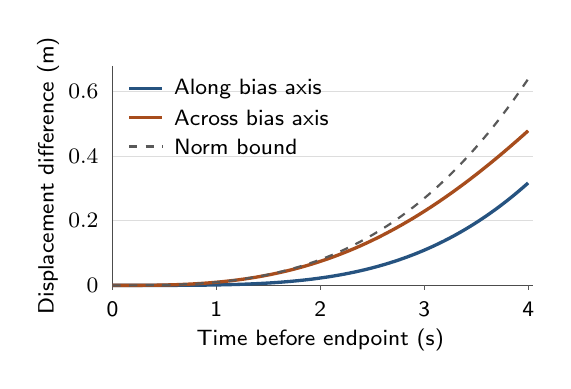
\begin{tikzpicture}[x=1.32cm,y=4.1cm,font=\sffamily\footnotesize]
  \definecolor{parallelblue}{RGB}{38,83,128}
  \definecolor{crossorange}{RGB}{167,77,29}
  \foreach \y in {0,.2,.4,.6}{
    \draw[gray!27] (0,\y)--(4.05,\y);
    \node[anchor=east] at (-.04,\y) {\pgfmathprintnumber[fixed,precision=1]{\y}};
  }
  \draw[black!70] (0,.68)--(0,0)--(4.05,0);
  \foreach \x in {0,1,2,3,4}{
    \draw[black!65] (\x,0)--(\x,-.015);
    \node[anchor=north] at (\x,-.02) {\x};
  }
  \node[rotate=90] at (-.62,.34) {Displacement difference (m)};
  \node[anchor=north] at (2,-.105) {Time before endpoint (s)};
  % Q(T-u) rotates the body x-axis by -omega*u, with omega = 0.60 rad/s.
  \draw[parallelblue,very thick,domain=0:4,samples=80]
    plot (\x,{.1*(\x*\x/2-(1-cos(deg(.6*\x)))/.36)});
  \draw[crossorange,very thick,domain=0:4,samples=80]
    plot (\x,{.1*(.6*\x-sin(deg(.6*\x)))/.36});
  \draw[black!65,thick,dashed,domain=0:4,samples=60]
    plot (\x,{.01*\x*\x*\x});
  \draw[parallelblue,very thick] (.16,.61)--(.48,.61);
  \node[right] at (.50,.61) {Along bias axis};
  \draw[crossorange,very thick] (.16,.52)--(.48,.52);
  \node[right] at (.50,.52) {Across bias axis};
  \draw[black!65,thick,dashed] (.16,.43)--(.48,.43);
  \node[right] at (.50,.43) {Norm bound};
\end{tikzpicture}
